\documentclass[11pt]{article}

\usepackage{graphicx}
%\usepackage{algorithmic}
%\usepackage{algorithm}
\usepackage{amssymb}
\usepackage{amsmath}
\usepackage{enumerate}
\usepackage[mathscr]{euscript}

\begin{document}

\pagenumbering{arabic}

\begin{center}
{\LARGE{\textbf{Computational Theories of Collaboration}}} \\
\Large\textsc{Ph.D. Comprehensive Exam} \\[1em]
\large\textnormal{Mohammad Shayganfar - mshayganfar@wpi.edu} \\
\large\textnormal{May, 26 2015}
\end{center}

\section{Introduction to Collaboration Theories}

The construction of computer systems that are intelligent, collaborative
problem-solving partners is an important goal for both the science of AI and its
application. There is no question that there is a need to make computer systems
better at helping us do what we use them to do. collaboration must be designed
into systems from the start; it cannot be patched on. To build collaborative sys-
tems, we need to identify the capabilities that must be added to individual
agents so that they can work with other agents
\cite{grosz:collaborative-systems}.

Most collaborative situations involve agents who have different beliefs and
capabilities. Partial knowledge is the rule, not the exception. As a result,
collaborative planning requires an ability to ascribe beliefs and intentions.

Another feature of collaborative activity is collaborative plans are not simply
the sum of individual plans.

To be collaborative, partners, e.g., a robot and a human, need to meet the
specifications stipulated by some theories that we review in this document. As
we discuss in Section \ref{sec:sharedplans}, collborators need to commit to the
group activity and to their role in it; they need to divide the task load
according to their capabilities so they can carry out the individual plans that
constitute the group activity; and they need to commit to the success of others.
Collaborators also need to be able to communicate with others effectively, and
to interpret others' actions and utterances in the collaboration context.
Furthermore, collaborators need to be willing to help others in doing their own
tasks, and to reconcile between commitments to existing collabortion and their
other activities \cite{grosz:mice-menus}.

Collaboration is a special type of coordinated activity in which the
participants work jointly, together performing a task or carrying out the
activities needed to satisfy a shared goal \cite{grosz:collaboration}.

Existing collaboration theories (including SharedPlans) consider the nature of a
collaboration to be more than a set of individual acts. These theories argue for
an essential distinction between a collaboration and a simple interaction or
even a coordination in terms of commitments \cite{grosz:shared-plans,
lochbaum:collaborative-planning}.

\section{Shared Activity}

Joint action can best be described as doing something as a team where the
participants share the same goal and a common plan of execution. Grosz and
Sidner has pointed out that collaborative plans do not reduce to the sum of the
individual plans \cite{grosz:plans-discourse}
\cite{grosz:collaborative-systems}.

For example, if we were to move a table jointly through a doorway, your picking
up one side of the table and starting to walk through the door does not make
sense outside our joint activity. Even the sum of both our picking-up and moving
actions would not amount to the shared activity without the existence of a
collaborative plan that both of us are sharing (namely to move the table out the
door). It seems that we both hold a joint intention, as well as individual
intentions related to this joint intention.

\section{Communication}

Cohen’s Joint Intention Theory predicts that an efficient and robust
collaboration scheme in a changing environment requires an open channel of
communication. Sharing information through communication acts is critical given
that each teammate often has only partial knowledge relevant to solving the
problem, different capabilities, and possibly diverging beliefs about the state
of the task.

\section{Teamwork \& Collaboration}

Bratman's view is that collective intention can be described by referring to
individual intention in combination with other mental attitudes. Searle's
opposing view is that collective intention cannot be so reduced.

According to Joint Intentions theory, the notion of teamwork is characterized by
joint commitment (also known as joint persistent goal or JPG). The definition of
JPG states that the agents mutually believe they have the appropriate goal, and
that they mutually believe a persistent weak achievement goal (which represents
the one-way commitment of one agent directed towards another) to achieve it
persists until the agents mutually believe that the goal has either been
achieved, impossible, or irrelevant.

\section{Computational Theories of Collaboration}

There are prominent collaboration theories that are mostly based on plans and
often analysis of the discourse between collaborators revolving around these
plans \cite{grosz:plans-discourse, Litman:discourse-commonsense}. In these
theories the discourse analysis is based on search over these tree plans
\cite{rich:discourse}.

The two theories Joint Intentions and SharedPlans have been extensively used to
examine and describe teamwork.

Two important theories for modeling teamwork collaboration were derived from
the BDI paradigm.

\subsection{Theory of Joint Intentions/Teamwork}

1. Mutual belief in the joint intention

2. Joint execution until MB in goal termination

3. Termination:

- Goal achieved

- Goal unachievable

- Goal irrelevant

[Use my own example] Supporting Bratman’s guidelines, Cohen and Levesque propose
a formal approach to building artificial collaborative agents. Their notion of
joint intention is viewed not only as a persistent commitment of the team to a
shared goal, but also implies a commitment on part of all its members to a
mutual belief about the state of the goal. Teammates are committed to inform the
team when they reach the conclusion that a goal is achievable, impossible, or
irrelevant. In our table-moving example, if one team member reaches the
conclusion that the table will not fit through the doorway, it is an essential
part of the implicit collaborative “contract”, to have an intention to make this
knowledge common. In a collaboration, agents can count on the commitment of
other members, first to the goal and then—if necessary—to the mutual belief of
the status of the goal.

The Joint Intentions Framework \cite{levesque:acting-together}
\cite{cohen:intention-commitment} \cite{cohen:persistence-intention-commitment}
is a theoretical framework founded on BDI logics. The framework focuses on a
team's joint mental state, called a joint intention. A team jointly intends a
team action if all team members are jointly committed to perform an action while
in a specified mental state.

According to this theory, joint action is conceptualized as doing something
together as a team where the teammates share the same goal and the same plan of
execution. Sharing information through communication acts is critical given that
each teammate often has only partial knowledge relevant to solving the problem,
different capabilities, and possibly diverging beliefs about the state of the
task. Communication plays an important role in coordinating their roles and
actions to accomplish the task. It also serves to establish and maintain a set
of mutual beliefs (also called common ground) among the team members. For
instance, all teammates need to establish and maintain a set of mutual beliefs
regarding the current state of the task, the respective roles and capabilities
of each member, the responsibilities of each teammate, etc. What happens when
things go wrong? Teammates must share a commitment to achieving the shared goal.
They cannot abandon their efforts, but must instead continue to coordinate their
efforts to try a different, mutually agreed upon plan. [--> Leonardo]

Joint Intentions Theory describes how a team of agents can jointly act together
by sharing mental states about their actions. An intention is viewed as a
commitment to perform an action while in a mental state. And a joint intention
is a shared commitment to perform an action while in a group mental state
\cite{cohen:intention-commitment}. Communication is required to establish and
maintain mutual beliefs and joint intentions. A team of agents jointly intend to
perform an action if and only if the members have a joint persistent goal
\cite{cohen:teamwork}.

In order to enter a joint commitment, the team members have to establish
appropriate mutual beliefs and individual commitments. Although the Joint
Intentions Theory does not mandate communication and several techniques are
available to establish mutual beliefs about actions from observations (see
\cite{huber:without-communication}), currently communication seems to be the
only feasible way to attain joint commitments. A key aspect of the Joint
Intention Theory is the commitment to attain mutual belief about the termination
of a team action. This helps to ensure that the team stays updated about the
status of the team actions. This behaviour is achieved by enforcing that agents
committing to a joint intention also commit to inform their team about any
relevant failures or premature terminations. Joint intentions and joint
commitments provide a basic framework to reason about coordination required for
teamwork as well as guidance for monitoring and maintaining team activities.
However, a single joint intention for a high-level team goal is not sufficient
to model team behaviour in detail and to ensure coherent teamwork.

There are also some other theories with similarities and contrasts conveying
collaboration concepts including Cohen and Levesque's work describing the
concept of \textit{joint intentions} in \cite{cohen:teamwork,
levesque:acting-together}.

In \cite{cohen:teamwork} Cohen and Levesque establish that joint intention
cannot be defined simply as individual intention with the team regarded as an
individual. This is because after the initial formation of an intention, team
members may diverge in their beliefs and hence in their attitudes towards the
intention. Instead, Cohen and Levesque generalise their own definition of
intention. First they present a definition of individual persistent goal and, in
terms of this, individual intention. Both definitions use the notion of
individual belief. Next, they define precise analogues of these concepts --
joint persistent goal and joint intention -- by invoking mutual belief in place
of individual belief. The definition of joint persistent goal additionally
requires each team member to commit to informing other members -- to the extent
of the team's mutual belief -- if it comes to believe that the common goal has
been achieved, becomes impossible or is no longer relevant. The result is that,
while a team is not an individual, nevertheless joint intention is similar to
individual intention. In Cohen and Levesque's theory, then, a team with a joint
intention is a group that shares a common objective and a certain shared mental
state. In particular, joint intentions are held by the team as a whole
\cite{jarvis:teams-multiagent-systems}.

\subsection{SharedPlans Theory}
\label{sec:sharedplans}

\subsubsection{Communicating Intentions}

Using discourse plans can help to encode the knowledge about conversation.

The SharedPlans theory recognises three interrelated levels of discourse
structure.

In \cite{grosz:plans-discourse}, Grosz and Sidner argue that the components of
the discourse structure are a trichotomy of linguistic structure, intentions
structure and the attention state. In their work, the linguistic structure of a
discourse is a sequence of utterances aggregating into discourse segments just
as the words in a single sentence form constituent phrases. They also discuss
the idea of the discourse purpose as the intention that underlies engagement in
the particular discourse. They believe this intention is the reason behind
performing a discourse rather than some other actions, and also the reason
behind conveying a particular content of the discourse rather than some other
contents. They describe mechanisms for plan analysis looking at Discourse
Segment Purposes (DSPs). In fact, the DSPs specify how the discourse segments
contribute to achieving the overall discourse purpose. Finally, the third
component in their theory, the attentional state, provides an abstraction of the
agent's focus of attention as the discourse unfolds. The focusing structure
contains DSPs and the stacking of focus spaces reflects the relative salience of
the entities in each space during the discourse. In short, the focusing
structure is the central repository for the contextual content required for
processing utterances during the discourse \cite{grosz:plans-discourse}.

\subsubsection{Collaboration Vs. Sum of Coordinate Actions}

\cite{grosz:collaborative-systems}

\subsubsection{SharedPlans}

Grosz and Sidner (1996) propose that collaboration must have three elements:

1. the participants must have commitment to the shared activity,

2. there must be a process for reaching an agreement on a recipe for the group
action, and

3. there must be commitment to the constituent actions.

The SharedPlans formalization distinguishes partial plans and complete plans. A
Full SharedPlan (FSP) is a complete plan in which agents have fully determined
how they will perform an action. The Partial SharedPlan (PSP) definition
provides a specification of the minimal mental-state requirements for
collaboration to exist and gives criteria governing the process of completing
the plan. Consequently, a full recipe for doing an action \textit{A} is a set of
actions and constraints such that the doing of those actions under those
constraints constitutes the doing of action \textit{A}. A partial recipe is a
set of actions and constraints that may be extended to a full recipe
\cite{grosz:planning-acting}.

Grosz and Sidner \cite{grosz:plans-discourse}
Grosz and Kraus \cite{grosz:collaboration}

SharedPlans is a general theory of collaborative planning that requires no
notion of joint intentions, accommodates multi-level action decomposition
hierarchies and allows the process of expanding and elaborating partial plans
into full plans.

SharedPlans is rooted in the observation that collaborative plans are not simply
a collection of individual plans, but rather a tight interleaving of mutual
beliefs and intentions of different team members.

The SharedPlans model of collaborative action \cite{grosz:planning-acting}
\cite{grosz:collaboration} \cite{grosz:plans-discourse} aims to provide the
theoretical foundations needed for building collaborative robots/ agents
\cite{grosz:collaborative-systems}. It specifies four key characteristics for
participants in a group activity to be collaborative partners, and thus for
their joint activity to be collaborative. The SharedPlans definition states that
for a group activity to be collaborative, the collaborators must have:

Look at this carefully!!!

\begin{enumerate}[a)]
  \item individual intentions that the group perform the group activity;
  \item mutual belief of a (partial or complete) recipe;
  \item individual or group plans for the constituent subactions of the recipe;
  \item intentions that their collaborators succeed in doing the constituent
  subactions.
\end{enumerate}
 
In other words, to successfully complete a plan the collaborators must mutually
believe that they have a common goal and have agreed on a sequence of actions
for achieving that goal. They should believe that they are both capable of
performing their own actions and intend to perform those actions while they are
committed to the success of their plans.

The intentions that this definition specifies constitute different kinds of
commitments required of the collaborators. 

The idea behind partial shared plans is enabling the agents to modify the shared
plan over the course of planning without impairing the achievement of the shared
goals.

\subsubsection{Intention-to and Intention-that}

In Grosz and Sidner's SharedPlans theory \cite{grosz:plans-discourse}, two
intentional attitudes are employed: ``intending to" (do an action) and
``intending that" (a proposition will hold). The notion of \textit{intention
to}, as an individual-oriented intention, models the intention of an agent to do
any single-agent action while the agent not only believes that it is able to
execute that action, but it also committs to doing so. In short, it is an
intention to perform an action, similar to Bratman’s conception. In contrast
with \textit{intention to}, an \textit{intention that}, as the notion of an
intention directed toward group activity, does not directly imply an action. In
fact, an individual agent's \textit{intention that} is directed towards its
collaborator's action or towards a group's joint action. \textit{Intention that}
guides an agent to take actions (including the communication), that enable or
facilitate other collaborators to perform assigned tasks. This leads an agent to
behave in a manner consistent with a collaborative effort. Therefore, agents
will adopt intentions to communicate about the plan \cite{grosz:collaboration}.
There is a significant difference between ``Intention that'' and ``Intention
to". ``Intention to" commits an agent to means-end reasoning and acting
\cite{bratman:intentions-plans}. In contrast, ``Intention that'' does not
necessarily entail this commitment.

\subsubsection{Recipes}

The SharedPlans definition of mutual beliefs states that when agents have a
shared plan for doing some act, they must hold mutual beliefs about the way in
which to perform that act. Following Pollack
\cite{pollack:plan-mental-attitudes}, the term recipe refers to what
collaborators know when they know a way of doing something. Recipes are
specified at a particular level of detail. Hence, the agents need to have mutual
beliefs about acts specified at the particular level of detail of the recipe,
and they do not to have mutual beliefs about all levels of acts that each agent
will perform. Mutual belief of the recipe essentially means that all the
collaborators hold the same beliefs about the way in which the activity will be
accomplished. Therefore, the collaborators must agree on how to do the activity.
Grosaz and Sidner in their earlier work \cite{grosz:plans-discourse} have
considered only simple recipes in which each recipe consisted of only a single
act-type relation \cite{lochbaum:plan-models}. Recipes are aggregations of
act-types and relations among them. Act-types, rather than actions, are the main
elements in recipes. Recipes can be partial, meaning thay can expand and be
modified over time.

\subsubsection{Plans}

Figure \ref{fig:plans} shows what we need to add to individual plans in order to
have plans for group action, and lists the major components of group plans; to
provide a base for comparison, the top of the figure lists the main components
for individual plans. First, just as an individual agent must know how to do an
action, agents in a group must have knowledge of how they’re going to do an
action. In the case of a group plan to do a joint activity, there must be mutual
belief of the recipe; agents must agree on how they are going to do the action.
Then, just as individual agents must have the ability to perform the constituent
actions in an individual plan and must have intentions to perform them, the
participants in a group activity must have individual or group plans for each of
the constituent actions in their agreed-on recipe \cite{grosz:plans-discourse}
\cite{grosz:collaborative-systems}.

\begin{figure}[tbh]
  \center
  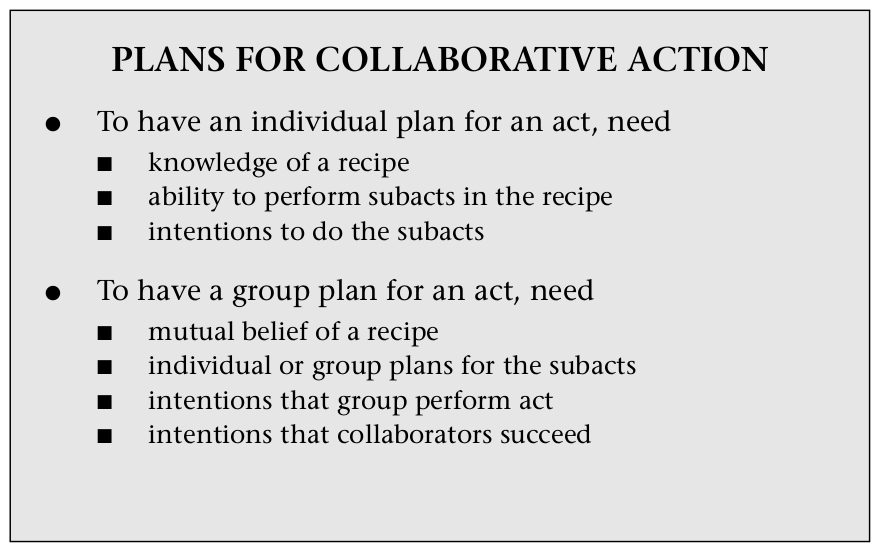
\includegraphics[width=0.9\textwidth]{figure/plans.png}
  \caption{Plans for collaborative action \cite{grosz:collaborative-systems}.}
  \label{fig:plans}
\end{figure}

Plans for group actions include two major constituents that do not have
correlates in the individual plan. First, the agents must have a commitment to
the group activity; they must all intend-that the group will do the action. For
instance, a robot and an astronaut need to have intentions that they install
solar panels. Among other things, these intentions will keep them both working
on the panels until the panels are installed. Second, the participants must have
some commitment to the other agents being able to do their actions. For example,
the robot must have an intention that the astronaut be able to measure the
quality of installation. This intention will prevent the robot from interrupting
astronaut's measurement action or prevent the robot from using astronaut's
measurement tool \cite{grosz:plans-discourse}
\cite{grosz:collaborative-systems}.

\subsubsection{Commitment}

Teamwork is:

Mutual commitment to joint activity:

- Agreement on the joint activity

- Cannot abomdom activity without involving teammates

Mutual suppport:

- Must be active in helping teammate activity

Mutual Responsiveness:

- Take over tasks from teammates if necessary

Joint Intentions theory is expressed in a modal language.

Individual Commitment:(Joint Intentions)

PGOAL (Persistent Goal) to achieve p relative to q

1. she believes that p is currently false.

2. she wants p to be true eventually.

3. 2. will continue to hold until she comes to believe that p is true, or will
never be true, or that q is false (q is irrelevance clause for the case that p
becomes unnecessary).

Joint Commitment: (Joint Intentions)

JPG (Joint Persistent Goal) to achieve p relative to q

1. they mutually believe that p is currently false.

2. they mutually believe that they all want p to be true eventually.

3. until they come to mutually believe that p is true, or will never be true, or
that q is false, they will continue to mutually believe that they each have p as
a AGOAL (Achievement Goal)

Joint Intention:

A Join Intention of team t to achieve p relative to q
≡
t’s members have a JPG to achieve p relative to q 
+
t’s members are believing throughout that they are doing it.

(a joint intention to perform a particular action is a joint commitment to enter
a future state wherein the agents mutually believe the collaborative action is
imminent just before they perform it)

Theorem:

If a team jointly intends to do a complex action consisting of team members
concurrently doing individual actions, then the individuals will privately
intend to do their share relative to the joint intention.

The notion of an agent’s commitment to achieving some state in the world is
expressed as a persistent goal or PGOAL in Joint Intentions Theory
\cite{cohen:intention-commitment}. An agent x has a persistent goal (PGOAL x p
q) if x wants p to become true and cannot give up the goal until it believes
that p is accomplished, or is impossible, or is irrelevant. An intention to do
an action is defined as a persistent goal in which the agent is committed to
performing the action believing throughout that it is doing that action.

Bratman in \cite{bratman:intentions-plans} has argued that intentions noramlly
pose the problems for the agent and agents needs to determine an action to
achieve those intentions. He also argued that intentions constrain an agent’s
choice of what else it can intend, and they provide the context for an agent’s
replanning when something goes wrong. The commitment to joint activity leads to
a need to communicate.

Finally, the definition of the overall plan in terms of constituent plans of
individuals or groups is recursive, with the recursion ending at the level of
basic, individual actions \cite{grosz:mice-menus}.

Grosz, Sidner and Lochbaum in \cite{grosz:plans-discourse} and
\cite{lochbaum:plan-models} present a model of plans to account for how agents
with partial knowledge collaborate in the construction of a domain plan. Agents
have a library of partially speci ed plan schemas (recipes). These recipes might
be underspeci ed as to how an action is executed or how an action contributes to
a goal. Agents then collaborate in constructing a shared plan by uttering
statements about their beliefs and intentions about the plan. This collaboration
will terminate with each agent mutually believing that each act in the plan can
be executed by one of the agents, that that agent intends to perform the act,
and that each act in the plan contributes to the goal.

Grosz, Sidner and Lochbaum in \cite{grosz:plans-discourse} and
\cite{lochbaum:plan-models} are interested in the type of plans that underlie
discourse in which the agents are collaborating in order to achieve a shared
goal. They propose that agents are building a shared plan in which participants
have a collection of beliefs and intentions about the actions in the plan.

Grosz, Sidner and Lochbaum in \cite{grosz:plans-discourse} and
\cite{lochbaum:plan-models} model how several agents with partial knowledge
collaborate on constructing a shared domain plan . Each agent communicates their
beliefs and intentions by making utterances about what actions they can
contribute to the shared plan. Collaboration is again modelled by the agents
establishing a mutual belief that each action in the shared plan contributes to
the goal of the plan, and that each action can and will be performed by one of
the agents.

\textit{Shared plan} is another essential concept in the collaboration context.
The definition of the shared plan is derived from the definition of plans
Pollack introduced in \cite{pollack:plan-inference,
pollack:plan-mental-attitudes} since it rests on a detailed treatment of the
relations among actions and it distinguishes the intentions and beliefs of an
agent about those actions. However, since Pollack's plan model is just a simple
plan of a single agent, Grosz and Sidner extended that to plans of two or more
collaborative agents. The concept of the shared plan provides a framework in
which to further evaluate and explore the roles that particular beliefs and
intentions play in collaborative activity \cite{lochbaum:plan-models}. However,
this formulation of shared plans (a) could only deal with activities that
directly decomposed into single-agent actions, (b) did not address the
requirement for the commitment of the agents to their joint activities, and (c)
did not adequately deal with agents having partial recipes
\cite{grosz:collaboration}. Grosz and Kraus in \cite{grosz:collaboration},
reformulate Pollack's definition of the individual plans
\cite{pollack:plan-mental-attitudes}, and also revise and expand the SharedPlans
to address these shortcomings.

\subsubsection{Coordinated Cultivation of SharedPlans}

Grosz and Hunsberger \cite{grosz:ccsp} claim to reconcile the two approaches.
They provide the ``Coordinated Cultivation of SharedPlans" (CCSP) model, which,
while relying solely on individual intention, captures the essential properties
argued for in accounts that require group-oriented intention. CCSP also provides
a general architecture for collaboration-capable agents.

\subsection{Hybrid Collaboration Approaches}

Building on the well developed theory of joint intentions \cite{cohen:teamwork}
and shared plans \cite{grosz:plans-discourse} \cite{grosz:collaboration}, the
STEAM teamwork model \cite{tambe:flexible-teamwork} was operationalized as a set
of domain independent rules that describe how teams should work together.

Tambe's work on \textit{STEAM teamwork model} \cite{tambe:flexible-teamwork}.

Jennings work in \cite{jennings:joint-intention-hybrid}

STEAM (Shell for Teamwork) builds on both Joint Intention Theory and Shared Plan
Theory and tries to overcome their shortcomings. Based on joint intentions,
STEAM builds up hierarchical structures that parallel the Shared Plan Theory as
described in the previous chapter. Hence, STEAM formalises commitments by
building an  maintaining Joint Intentions, and uses SharedPlans to formulate the
team's attitudes in complex tasks.

In \cite{tambe:flexible-teamwork} Tambe presents STEAM, an implemented model of
teamwork based primarily on Cohen et al.'s theory of Joint Intentions, but
informed by key concepts from SharedPlans. Following Cohen et al., a team
initially adopts a joint intention for a high-level team goal that includes
commitments to maintain the goal until it is deemed already achieved,
unachievable or irrelevant. The agents then construct a hierarchy of individual
and joint intentions analogous to partial SharedPlans. Tambe notes that as the
hierarchy evolves, if a step involves only a subteam then that subteam must form
a joint intention to perform that step, and the remaining team members need only
track the subteam's joint intention, requiring that they be able to infer
whether or not the subteam intends to, or is able to, execute that step
\cite{hunsberger:shared-plans-easier}.

\section{Relation to Psychology and Sociology}

[from Hoffman \& Breazeal] In Bratman’s detailed analysis of Shared Cooperative
Activity (SCA), he defines certain prerequisites for an activity to be
considered shared and cooperative: he stresses the importance of mutual
responsiveness, commitment to the joint activity and commitment to mutual
support. His work also introduces the idea of meshing singular sub-plans into a
joint activity. In our implementation, we generalize this concept to the idea of
dynamically meshing sub-plans.

Referring expressions \cite{heeman:model-collaboration-referring}

\section{Similarities and Differences}

- SharedPlans theory:

+ Teammates agree on SharedPlan

+ Plan it together, execute it together

+ Specifies conditions for assistance, monitoring

- Joint Intentions theory

+ Teammates agree on intentions

+ Teammates agree on selecting/deselecting goals

+ i.e., goal unachievable, achieved, irrelevant

Similar to SharedPlans theory by Grosz and Sidner, Joint Intentions theory
specifies what it means for agents to execute actions as a team.
\cite{subramanian:joint-intention-dialogue}.

Cohen and Levesque Joint Intentions theory also states that a joint action could
not be seen as a collection of individual ones but that agents working together
need to share belief.

\begin{enumerate}
  \item None of SharedPlans' four components (see Section \ref{sec:sharedplans})
  has the notion of a joint intention. This is a significant difference between
  SharedPlans and Joint Intentions theories, since the notion of joint intention
  is an integral part of Cohen and Levesque's theory. In particular, SharedPLans
  theories emphesizes on the agents individually intending that the joint action
  be done successfully as well as the agents individually intending the success
  of their collaborators' actions which is introduced in
  \cite{grosz:collaboration} by Grosz and Kraus as the notion of
  \textit{intention-that}.
  \item Communication requirements are derived from any intention that's, as
  opposed to being ``hard-wired" in Joint Intentions.
  \item In contrast to Joint Intentions, the SharedPlans Theory employs
  hierarchical structures over intentions, thus overcoming the shortcoming of a
  single Joint Intention for complex team tasks. The Shared Plans Theory is not
  based on a joint mental attitude but on an intentional attitude called
  intending that, which is very similar to an agent’s normal intention to
  perform an action.
  \item Another main difference between the Joint Intentions Theory and the
  SharedPlans Theory is that the Shared Plans Theory describes the way to
  achieve a common goal through the hierarchy of plans, whereas the Joint
  Intentions Theory describes only this common goal
  \cite{skubch:modelling-behavior-robots}.
  \item Joint Intentions theory assumes that knowledge about the team-mates is
  always available.
\end{enumerate}

\section{Application in Human-Computer Collaboration}

COLLAGEN \cite{rich:collaboration-manager,rich:discourse} is the first
implemented system based on the SharedPlans theory. It incorporates certain
algorithms for discourse generation and interpretation, and is able to maintain
a segmented interaction history, which facilitates the discourse between human
user and the intelligent agent. The model includes two main parts: (1) a
representation of discourse state and (2) a discourse interpretation algorithm
utterances of the user and agent \cite{rickel:discourse-theory-dialogue}.

In \cite{heeman:model-collaboration-referring} Heeman presents a computational
model of how a conversational participant collaborates in order to make a
referring action successful. The model is based on the view of language as
goal-directed behaviour, and in his work, he refers to SharedPlans as part of
the planning and conversation literature.

In \cite{lochbaum:plan-models}, Lochbaum and Sidner modify and expand the
SharedPlan model of collaborative behavior \cite{grosz:plans-discourse}. They
present an algorithm for updating an agent’s beliefs about a partial SharedPlan
and describe an initial implementation of this algorithm in the domain of
network management.

The system GRATE* by Jennings \cite{jennings:joint-intention-hybrid} is based on
the Joint Intention Theory. GRATE* provides a rule-based modelling approach to
cooperation using the notion of Joint Responsibilities, which in turn is based
on Join Intentions. GRATE* is geared towards industrial settings in which both
agents and the communication between them can be considered to be reliable.

CAST (Collaborative Agents for Simulating Teamwork) \cite{yen:cast}
\cite{yin:knowledge-based-sharedplans} is a teamwork framework based on the
SharedPlans Theory. CAST focuses on flexibility in dynamic environments and on
proactive information exchange enabled by anticipating what information team
members will need. Petri Nets are used to represent both the team structure and
the teamwork process, i.e., the plans to be executed.

Researchers in \cite{hobbs:microsociology-relationship} discuss developing an
ontology of microsocial concepts for use in an instructional system for teaching
cross-cultural communication. They believe being acquainted with one another is
not a strong enough relationship to create a society from. Hence, there is a
need for commitment and shared plans (as the basis of social life) to achieve a
shared goal. In this work, Gorsz and Sidner's SharedPlans theory
\cite{grosz:plans-discourse} is used to explain the concept of shared plans
within the interpersonal relationships of societies in an industrial
environment.

In \cite{hunsberger:auction-collaborative} Hunsberger and Grosz discuss the idea
of whether the rational, utility-maximizing agents should determine commiting to
a group activity when there is an opportunity to collaborate. They call this
problem as the ``initial-commitment decision problem'' (ICDP) and provide a
mechanism that agents can use to dolve the ICDP. They use the representation of
action, act-types and recepies in the SharedPlans theory.

In \cite{zamfirescu:gdss} an integrated agent-based model for Group Decision
Support Systems is proposed and discussed. The decisional model that authors
outline in this paper is based on the SharedPlans theory.

Rauenbusch and Grosz in \cite{rauenbusch:decision-making-planning} formally
define a search problem with search operators that correspond to the team
planning decisions. They provide an algorithm for making the three types of
interrelated decisions by recasting the problem as a search problem. Their model
respects the constraints on mental states specified by the SharedPlans theory of
collaboration.

In \cite{marsella:robocup} authors provide their in RoboCup (robotics soccer
testbed) in which their focus is on teamwork and learning challenges. Their
research investigationin RobotCup is based on ISI Synthetic, a team of synthetic
soccer-players. They also investigate the use of STEAM as their model of
teamwork which is influenced by the Joint Intentions and SharedPlans theories.

Babaian et. al. ini \cite{babaian:writers-assistant} describe Writer’s Aid, a
system that deploys AI planning techniques to enable it to serve as an author’s
collaborative assistant. While an author writes a document, Writer’s Aid helps
in identifying and inserting citation keys and by autonomously finding and
caching potentially relevant papers and their associated bibliographic
information from various on-line sources. They believe the underlying concepts
of SharedPlans is relevent since in collaborative interfaces like Writer’s Aid,
the users establish shared goals with the system and user and the system
both take initiative in satisfying them.

In \cite{montreuil:planning-robot-activity} researchers address high-level robot
planning issues for an interactive cognitive robot that acts in presence or in
collaboration with a human partner. They describe a Human Aware Task Planner
(HATP) which is designed to provide socially acceptable plans to achieve
collaborative tasks. They use notions of plans based on SharedPlans theory.

In \cite{sidner:enagagement-robot} Sidner and Dzikovska argue that robots, in
order to participate in conversations with humans, need to make use of
conventions of conversation and the means to be connected to their human
counterparts. They provide an initial research on engagement in human-human
interaction and applications to stationary robots in hosting activities. They
believe hosting activities are collaborative because neither party completely
determines the goals to be undertaken nor the means of reaching the goal. To
build a robot host, they rely on an agent built using Collagen which is
implemented based on the SharedPlans theory.

In \cite{kinny:planned-team} authors introduce a language for representing joint
plans for teams of agents. They describe how agents can organize the formation
of a suitably skilled team to achieve a joint goal, and they explain how such a
team can execute these plans to generate complex, synchronized team activity. In
this paper, authors adopt the underlying concepts of the Joint Intentions theory
as the structure of their collaborative agents.

Breazeal et. al. in \cite{breazeal:humanoid-robots} present an overview of their
work towards building socially intelligent, cooperative humanoid robots,
Leonardo, that can collaborate and learn in partnership with humans. They employ
the Joint Intentions theory of collaboration to implement the collaborative
behaviors while performing a task in collaboration with humans.

In \cite{subramanian:joint-intention-dialogue} researchers' goal is to develop
an architecture (based on the concepts of Joint Intentions theory) that can
guide an agent during collaborative teamwork. They describe how a joint
intention interpreter that is integrated with a reasoner over beliefs and
communicative acts can form the core of a dialogue engine. Ultimately, the
system engages in dialogue through the planning and execution of communicative
acts necessary to attain the collaborative task at hand.

Mutlu et. al. in \cite{mutlu:coordination-robot} discuss key mechanisms for
effective coordination toward informing the design of communication and
coordination mechanisms for robots. They present two illustrative studies that
explore how robot behavior might be designed to employ these mechanisms
(particularly joint attention and action observation) to improve measure of task
performance in human-robot collaboration. Their work uses Joint Intentions
theory to develop shared task representations and strategies for task
decomposition.

In \cite{kabil:coordination-mechanisms} researchers propose a behavioral
architecture C2BDI that allows to enhance the knowledge sharing using natural
language communication between team members. They define collaborative
conversation protocols that provide proactive behavior to agents for the
coordination between team members. Their agent architecture provides
deliberative and conversational behaviors for collaboration, and it is based
on both of the SharedPlans and Joint Intentions theories.

This domain independent teamwork model, STEAM, has been successfully applied to
a variety of domains.  From combat air missions
\cite{hill:synthetic-battlefield-aircraft} to robot soccer \cite{kitano:robocup}
to teams supporting human organizations
\cite{pynadath:teamwork-heterogeneous-agents} to rescue response
\cite{scerri:robot-agent-person}, applying the same set of STEAM rules has
resulted in successful coordination between heterogeneous agents. The successful
use of the same teamwork model in a wide variety of diverse domains provides
compelling evidence that it is the principles of team- work, rather than
exploitation of speciØc domain phenomena, that underlies the success of teamwork
based approaches.

There are many research focusing
on different aspects of collaboration each of which are different than my own
work. In my thesis, I focus on emotion functions and how they impact
collaboration's structure and processes, and how the dynamics of the
collaboration structure influences emotion-regulated processes. Some of the
other works focus on the concepts of robot assistants
\cite{clancey:agent-assistants-collaboration}, or teamwork and its challenges in
cognitive and behavioral levels \cite{cohen:teamwork,
nikolaidis:collaboration-joint-action, scerri:prototype-distributed-teams,
tambe:flexible-teamwork}. Some researchers have an overall look at a
collaboration concept at the architectural level. In
\cite{garcia:collaboration-emotional-awareness} authors present a collaborative
architecture, COCHI, to support the concept of emotional awareness. In
\cite{esau:integrating-emotion-collaboration} authors present the integration of
emotional competence into a cognitive architecture which runs on a robot, MEXI.
In \cite{sofge:collaboration-humanoid-space} authors discuss the challenges of
integrating natural language, gesture understanding and spatial reasoning of a
collaborative humanoid robot situated in the space. The importance of
communication during collaboration has been considered by some researchers from
human-computer interaction and human-robot collaboration
\cite{clair:action-intention-collaboraiton,
matignon:verbal-nonverbal-collaboration, rich:discourse} to theories describing
collaborative negotiation, and discourse planning and structures
\cite{andriessen:disourse-planning, grosz:discourse-structure,
sidner:discourse-collaborative-negotiation}. There are other concepts such as
joint actions and commitments \cite{grosz:intention-dynamics-collaboration},
dynamics of intentions during collaboration \cite{levesque:acting-together}, and
task-based planning providing more depth in the context of collaboration
\cite{burghart:cognitive-architecture-robot, rich:cea}.

The concept of collaboration has also received attention in the industry and in
research in robotic laboratories \cite{green:collaboration-literature-review}.

\section{Conclusion}

\bibliographystyle{plain}
\bibliography{mshayganfar}

\end{document}
